%; whizzy chapter
% -initex iniptex -latex platex -format platex -bibtex jbibtex -fmt fmt
% 以上 whizzytex を使用する場合の設定。


%     Tokyo Debian Meeting resources
%     Copyright (C) 2009 Junichi Uekawa
%     Copyright (C) 2013 Nobuhiro Iwamatsu

%     This program is free software; you can redistribute it and/or modify
%     it under the terms of the GNU General Public License as published by
%     the Free Software Foundation; either version 2 of the License, or
%     (at your option) any later version.

%     This program is distributed in the hope that it will be useful,
%     but WITHOUT ANY WARRANTY; without even the implied warranty of
%     MERCHANTABILITY or FITNESS FOR A PARTICULAR PURPOSE.  See the
%     GNU General Public License for more details.

%     You should have received a copy of the GNU General Public License
%     along with this program; if not, write to the Free Software
%     Foundation, Inc., 51 Franklin St, Fifth Floor, Boston, MA  02110-1301 USA

%  preview (shell-command (concat "evince " (replace-regexp-in-string "tex$" "pdf"(buffer-file-name)) "&"))
% 画像ファイルを処理するためにはebbを利用してboundingboxを作成。
%(shell-command "cd image200901; ebb *.png")

%%ここからヘッダ開始。

\documentclass[mingoth,a4paper]{jsarticle}
\usepackage{monthlyreport}
\usepackage{iwamatsu}

% 日付を定義する、毎月変わります。
\newcommand{\debmtgyear}{2013}
\newcommand{\debmtgmonth}{2}
\newcommand{\debmtgdate}{9}
\newcommand{\debmtgnumber}{1}


\begin{document}

\begin{titlepage}
\thispagestyle{empty}

% タイトルページ:編集必要な部分は最初のマクロに飛ばすこと

\vspace*{-2cm}
第\debmtgnumber{}回 Debian パッケージング道場資料

\hspace*{-2.4cm}
\includegraphics[width=210mm]{image200801/2008title.eps}\\
\hfill{}\debmtgyear{}年\debmtgmonth{}月\debmtgdate{}日

\end{titlepage}

\dancersection{Introduction}{上川 純一}

 今月のDebian勉強会へようこそ。これからDebianの世界にあしを踏み入れると
 いう方も、すでにどっぷりとつかっているという方も、月に一回Debianについ
 て語りませんか?

 Debian勉強会の目的は下記です。

 \begin{itemize}
 \item \underline{Debian Developer} (開発者)の育成。
 \item 日本語での「\underline{開発に関する情報}」を整理してまとめ、アップデートする。
 \item \underline{場}の提供。
 \begin{itemize}
  \item 普段ばらばらな場所にいる人々が face-to-face で出会える場を提供
	する。
  \item Debian のためになることを語る場を提供する。
  \item Debianについて語る場を提供する。
 \end{itemize}
 \end{itemize}		

 Debianの勉強会ということで究極的には参加者全員がDebian Packageをがりがり
 と作るスーパーハッカーになった姿を妄想しています。情報の共有・活用を通し
 て Debianの今後の能動的な展開への土台として、「場」としての空間を提供す
 るのが目的です。

\dancersection{基本的なパッケージの作成方法手引書}{岩松 信洋}
\subsection{本日の目的}

Debianパッケージ化されていないソフトウェアをパッケージ化して、
ビルドテストとパッケージの変更までを体験してみましょう。

\subsection{本日の流れ}
\begin{enumerate}
%\item Debian とは?
%\item Debian パッケージについて
\item 作業を始める前の準備をする
\item ソフトウェアの動作確認をする
\item パッケージの雛形を作成する
\item debian ディレクトリ以下ファイルを編集する
\item パッケージをビルドする
\item 作成されたファイルを見る
\item パッケージをインストールする
\item パッケージをビルドテストする
\item パッケージのインストール/アンインストールテストをする
\item ソフトウェアの変更し、パッケージ化する
\item 質疑応答
\end{enumerate}

\subsubsection{記号の説明}
{\bf \$} が付いている場合は、コンソールからの入力を意味します。{\bf \$}は入力せずに
コマンドを入力してください。

コマンドラインやファイルの中身で{\bf \textbackslash}が書かれている場所は行が続いて
いる事を意味します。入力しないでください。 

{\bf ...}は省略を意味します。実際には長い出力がある場合に省略している場
合に利用しています。

\subsection{ルート権限について}
本ハンズオンでは、root権限を使った作業を行う場合があります。
その場合には sudo コマンドを使って作業をします。{\bf sudo}コマンドが必要な場
合にはコマンドラインの説明のところに{\bf sudo}を指定しています。

\subsection{Debianとは}
省略

\subsection{Debian パッケージについて}
省略

\subsection{作業を始める前の準備をする}
 
\subsubsection{パッケージメンテナ名の設定}
パッケージメンテナの名前とメールアドレスを環境変数に設定します。
適当なエディタを使って、{\bf $\sim$/.bashrc} に以下の例のように追記して
保存してください。各項目には自分の名前とメールアドレスをいれてくだ
さい。
\begin{commandline}
export DEBFULLNAME="Nobuhiro Iwamatsu"
export DEBEMAIL=iwamatsu@debian.org
\end{commandline}
保存できたら、ターミナルを起動し、
\begin{commandline}
$ source ~/.bashrc
\end{commandline}
%$
を実行してください。

\subsubsection{パッケージビルドに必要なパッケージのインストール}

パッケージビルドに必要なパッケージのインストールをします。
{\bf packaging-dev}パッケージをインストールしてください。

\begin{commandline}
$ sudo apt-get install packaging-dev
\end{commandline}
%$

{\bf packaging-dev} はメタパッケージ\footnote{他のパッケージに依存するだけのパッケージ}
で、インストールすることによってDebianパッケージに必要なパッケージがインストールされます。

\begin{itemize}
\item build-essential\\
パッケージ作成環境にインストールされていることが前提となっているパッケージ
を提供するメタパッケージです。gcc、g++、 make 等を提供します。
 
\item debhelper\\
パッケージ作成補助ツールです。
\item devscripts\\
パッケージをメンテナンスするときに有用なスクリプトを提供します。
\item dput または dupload\\
パッケージのアップロードをする際に使用します。
\item lintian\\
パッケージを分析し、バグやポリシー違反を検出するツールです。
\item pbuilder または cowbuilder または sbuild\\
クリーンルームからパッケージを作成するための機能を提供します。
\item quilt\\
パッチ管理ツールです。
\end{itemize}

\subsubsection{パッケージ化するソフトウェア}
今回は、{\bf cwidget}を使ったサンプルプログラム
{\bf \url{http://people.debian.org/~iwamatsu/dpd/hello-cwidget-20120922.tar.gz}}
を用意しました。
このソフトウェアをDebianパッケージ化します。
ダウンロードして、適当なディレクトリに展開します。
\begin{commandline}
$ mkdir -p ~/debian/dojo/work
$ cd ~/debian/dojo/work
$ wget http://people.debian.org/~iwamatsu/dpd/hello-cwidget-20120922.tar.gz
$ tar -xzf hello-cwidget-20120922.tar.gz
$ ls
hello-cwidget-20120922.tar.gz
hello-cwidget-20120922
\end{commandline}
%$

このソフトウェアは C++ で記述されており、コンパイルに必要なソフトウェアやライブラリ
がインストールされている場合には、{\bf ./configure ; make ; sudo make install} 
を実行することでコンパイルおよびインストールまでができるようになっています。

\subsection{ソフトウェアの動作確認をする}

%\subsubsection{ソースを読んでみる}
%どのようなソフトウェアなのか理解するためにもパッケージ化する前に
%ソースコードを読んで、ソフトウェアの中身を理解しておきましょう。

\subsubsection{ソフトウェアをコンパイルしてみる}

コンパイルできない/動作しないプログラムをパッケージ化してもしょうがないので、動作確認をします。
まずは最低限コンパイルに必要なパッケージをインストールする必要
があります。それが{\bf build-essential}パッケージです。これはパッケー
ジ化の場合にも必要です。インストールしていない場合には以下のように実行して
インストールしてください。

\begin{commandline}
$ sudo apt-get install build-essential
\end{commandline}
%$

先ほど解凍したディレクトリに移動します。移動した後、{\bf configure}を実
行します。
\begin{commandline}
$ cd hello-cwidget-20120922
$ ./configure
...
Alternatively, you may set the environment variables \
SIGC_CFLAGS
and SIGC_LIBS to avoid the need to call pkg-config.
See the pkg-config man page for more details.
...
\end{commandline}
%$

実行するとエラーになります。ログを見てみると、{\bf pkg-config}コマンドが
なくてエラーになっている事がわかります。さて、{\bf pkg-config}コマンド
はどのパッケージで提供されているのでしょうか。

\subsection{提供されているパッケージを探す}

Debianで、特定のコマンドやファイルが提供されているパッケージを探すには、
{\bf apt-file}コマンドを利用します。apt-file コマンドは{\bf apt-file}パッケージで
提供されているのでインストールしておきましょう。インストールしたら検索用の
データベースを構築します。

\begin{commandline}
$ sudo apt-get update
$ sudo apt-get install apt-file
$ sudo apt-file update
\end{commandline}
%$

今回は{\bf pkg-config}コマンドがないので以下のように実行し、パッケージを
検索します。

\begin{commandline}
$ apt-file search pkg-config
pkg-config: /usr/bin/pkg-config
pkg-config: /usr/share/doc/pkg-config/AUTHORS
pkg-config: /usr/share/doc/pkg-config/NEWS.gz
.....
ruby-pkg-config: /usr/share/doc/ruby-pkg-config/copyright
zsh: /usr/share/zsh/functions/Completion/Unix/_pkg-config
zsh-beta: /usr/share/zsh-beta/functions/Completion/Unix/_pkg-config
\end{commandline}
%$


また、検索探したいファイルのパスがわかっている場合には、パスを指定して検索できます
(例: apt-file search /usr/bin/pkg-config)。

実行すると、指定したファイルを提供しているパッケージ名が出力されます。
結果を確認すると、{\bf pkg-config}パッケージで提供されていることが分かります。
{\bf pkg-config} コマンドが提供されているパッケージが{\bf pkg-config}パッケージとわかったので、
インストールします。

\begin{commandline}
$ sudo apt-get install pkg-config
\end{commandline}
%$

再度{\bf configure}を実行してみましょう。
\begin{commandline}
$ ./configure
...
No package 'sigc++-2.0' found

Consider adjusting the PKG_CONFIG_PATH environment variable if you
installed software in a non-standard prefix.
...
\end{commandline}
%$

次は{\bf sigc++-2.0}が見つからないようです。エラーメッセージを見ると
pkg-config を使って{\bf sigc++-2.0}の情報を取得しようとしているようですが、
見つからないためエラーになっていることが分かります。
\footnote{わからない人もいると思いますが。}

先ほどと同じように{\bf apt-file}を
利用して検索し、インストールします。

\begin{commandline}
$ apt-file search sigc++-2.0.pc
libsigc++-2.0-dev: /usr/lib/x86_64-linux-gnu/pkgconfig/sigc++-2.0.pc
$ sudo apt-get install libsigc++-2.0-dev 
\end{commandline}
%$

再度 configure を実行します。

\begin{commandline}
$ ./configure
...
checking for CWIDGET... configure: error: Package \
  requirements(cwidget) were not met:

No package 'cwidget' found

Consider adjusting the PKG_CONFIG_PATH environment variable if you
installed software in a non-standard prefix.
...
\end{commandline}
%$

また、エラーになります。今度は{\bf cwidget}足りないようなので、再度検索して
インストールします。

\begin{commandline}
$ apt-file search cwidget.pc
libcwidget-dev: /usr/lib/pkgconfig/cwidget.pc
$ sudo apt-get install libcwidget-dev
\end{commandline}

\begin{commandline}
$ ./configure
config.status: creating Makefile
config.status: creating config.h
config.status: config.h is unchanged
config.status: executing depfiles commands
\end{commandline}
%$

{\bf configure}が正常に終了しました。終了すると、{\bf Makefile}が
作成されています。{\bf make}を実行し、コンパイルします。

\begin{commandline}
$ make
make  all-am
make[1]: ディレクトリ `/home/iwamatsu/debian/dojo/work/hello-cwidget-20120922' に入ります
g++ -DHAVE_CONFIG_H -I.    -I/usr/include/sigc++-2.0 -I/usr/lib/x86_64-linux-gnu/sigc++-2.0/include   -I/usr/include/sigc++-2.0 -I/usr/lib/x86_64-linux-gnu/sigc++-2.0/include -I/usr/lib/cwidget   -g -O2 -MT hello_cwidget-hello-cwidget.o -MD -MP -MF .deps/hello_cwidget-hello-cwidget.Tpo -c -o hello_cwidget-hello-cwidget.o `test -f 'hello-cwidget.cc' || echo './'`hello-cwidget.cc
mv -f .deps/hello_cwidget-hello-cwidget.Tpo .deps/hello_cwidget-hello-cwidget.Po
g++ -I/usr/include/sigc++-2.0 -I/usr/lib/x86_64-linux-gnu/sigc++-2.0/include   -I/usr/include/sigc++-2.0 -I/usr/lib/x86_64-linux-gnu/sigc++-2.0/include -I/usr/lib/cwidget   -g -O2   -o hello-cwidget hello_cwidget-hello-cwidget.o -lsigc-2.0   -lcwidget -lncursesw -lsigc-2.0   
make[1]: ディレクトリ `/home/iwamatsu/debian/dojo/work/hello-cwidget-20120922' から出ます
\end{commandline}
%$

コンパイルも正常に終了したので、試しに実行します。
\begin{commandline}
$ ./hello-cwidget
\end{commandline}
%$

図のような画面が表示されたでしょうか。

\begin{center}
\includegraphics[width=0.5\hsize]{image201209/hello-debain.eps}
\end{center}

ここまではサンプルプログラムの動作確認です。先にどのようなソフトウェアな
のか理解するためにもパッケージング化する前にソースコード等を読んでおくこ
とをお勧めします。

\subsection{Debianパッケージの雛形を作成する}

Debianパッケージはソースが格納されているディレクトリの中に
{\bf debian}ディレクトリを作成し、その中にパッケージビルド用の
スクリプトを置き、実行することによってビルドされます。
これらを構成するファイルやスクリプトはある程度決まっているため、
雛形が用意されています。
この雛形を作成するのが{\bf dh\_make}コマンドで、{\bf dh\_make}は
{\bf dh-make}パッケージで提供されています。

今まで行った ./configure コマンド等で不要なファイルが作成されているため、
作業の前に一度{\bf hello-cwidget-20120922}ディレクトリを削除します。
そして再度展開し、作成されたディレクトリに移動します。

\begin{commandline}
$ cd ..
$ rm -rf hello-cwidget-20120922
$ tar -xzf hello-cwidget-20120922.tar.gz
$ cd hello-cwidget-20120922
\end{commandline}

以下のコマンドを実行し、{\bf dh-make}パッケージをインストールします。

\begin{commandline}
$ sudo apt-get install dh-make
\end{commandline}
%$

雛形の作成は以下のコマンドを実行します。
\begin{commandline}
$ dh_make --createorig -s
\end{commandline}
%$

{\bf \texttt{--}createorig}オプションはオリジナルソースコードのtar.gzイメージを構築し
ます。 今回はシングルバイナリパッケージ(一つのソースコードから一つの
バイナリパッケージがビルドされる)なので{\bf -s} を指定します。実行すると以下
のようなメッセージが表示されるので、Enterキーを押します。

\begin{commandline}
Maintainer name  : Nobuhiro Iwamatsu
Email-Address    : iwamatsu@debian.org 
Date             : Wed, 12 Sep 2012 12:46:24 +0900
Package Name     : hello-cwidget
Version          : 20120922
License          : blank
Type of Package  : Single
Hit <enter> to confirm: 
\end{commandline}

\subsubsection{debianディレクトリ}
コマンドを実行すると、{\bf debianディレクトリ}が作成され、この中に
パッケージ作成に必要な雛形が作成されます。
以下に作成されるファイル一覧を示します。

\begin{itemize}
\item README.Debian  (Debianパッケージの README)
\item README.source  (ソースの情報を記述する)
\item changelog      (Debianパッケージのチェンジログ)
\item compat         (debhelperのAPIバージョンを指定する)
\item control        (Debianパッケージ情報)
\item copyright      (著作権情報)
\item dirs           (作成するディレクトリ名を指定する)
\item docs           (インストールするドキュメントファイルを指定する)
\item emacsen-install.ex (emacs 用設定ファイル)
\item emacsen-remove.ex  (emacs 用設定ファイル)
\item emacsen-startup.ex (emacs 用設定ファイル)
\item hello-cwidget.cron.d.ex (cron用)
\item hello-cwidget.default.ex (debfonf用)
\item hello-cwidget.doc-base.EX (doc-base用)
\item init.d.ex      (init.dを使うパッケージ用設定ファイル)
\item manpage.1.ex   (manpage の雛形)
\item manpage.sgml.ex(manpage の雛形)
\item manpage.xml.ex (manpage の雛形)
\item menu.ex        (メニューの雛形)
\item postinst.ex    (postinstメンテナファイルの雛形)
\item postrm.ex      (postrmメンテナファイルの雛形)
\item preinst.ex     (preinstメンテナファイルの雛形)
\item prerm.ex       (prermメンテナファイルの雛形)
\item rules          (パッケージビルドスクリプト)
\item source         (Debian ソースパッケージ情報を格納するディレクトリ)
\item format     (Debian ソースフォーマットを指定する)
\item watch.ex       (アップストリームチェック用ファイル)

\end{itemize}

\subsubsection{不要なファイルの削除}
今回のパッケージ化に必要ではないファイルを{\bf debian}ディレクトリ以下から削除
します。hello-cwidget は emacs や cron を使わないプログラムなので、基本ファイルのみ
(changelog、compat、control、copyright、rules、source)のみでよいでしょう。
またサフィックスに .exと.EX がついてるファイルを使用する場合、サフィックスを
取り除いて内容を編集する必要があります(例: watch.ex $\rightarrow$ watch)。
\footnote{必須ファイルはchangelog、control、copyright、rules です。}

\begin{commandline}
$ rm -rf debian/*.ex debian/*.EX debian/README.Debian debian/README.source debian/dirs debian/docs
\end{commandline}
%$

\subsection{debian ディレクトリ以下ファイルの編集}

\subsubsection{debian/changelogファイルの編集する}

Debian パッケージの変更は全て簡潔に Debian changelog ファイル(debian/changelog)
に記載する必要があります。フォーマットに関しては
Debian policy 4.4 Debian changelog: debian/changelog を参照してください。
{\bf debian/changelog}ファイルには既に{\bf ITP}(Intent To Package)
\footnote{http://www.debian.or.jp/community/devel/abbreviation.html}
のテンプレート書かれているので削除します。以下のように変更します。

\begin{commandline}
hello-cwidget (20120922-1) unstable; urgency=low

  * Initial release.

 -- Nobuhiro Iwamatsu <iwamatsu@debian.org>  Wed, 12 Sep 2012 12:46:24 +0900

\end{commandline}
%$

\subsubsection{ライセンスとコピーライトをチェックする}

ソフトウェアをDebianパッケージにしてDebian にインストールする際、重要な点として
ソフトウェアのライセンスがあります。
そのソフトウェアのライセンスがDFSG(Debian Free Software Guideline)に適合するか
チェックする必要があり、同梱されているファイルを確認する必要があります。
ほとんどの場合、ソースにはLICENCEファイルやCOPYINGファイルが提供されていますが、
一部のファイルは違うライセンスが適用されている場合もあるためです。もちろんファイル毎に
ライセンスが書かれておらず、LICENCEファイル等で包容的にライセンスを決めている場合
もあります。

Debianでは簡易的にチェックするためのツールとして {\bf licensecheck}があります。
実行するとファイルのライセンスを出力します。
{\bf \texttt{--}copyright}オプションをつけた場合、コピーライトホルダも出力します。
{\bf -r}オプションは再帰チェックです。

\begin{commandline}
$ licensecheck -r .
hello-cwidget.cc: BSD (2 clause) 
$ licensecheck -r --copyright .
hello-cwidget.cc: BSD (2 clause) 
  [Copyright: HOLDERS AND CONTRIBUTORS / 2012 Nobuhiro Iwamatsu <iwamatsu@debian.org>]
\end{commandline}
%$

簡易的ではありますが hello-cwidget で提供されている hello-cwidget.cc
のライセンスは {\bf 2 clause BSD License}で、コピーライトは {\bf 2012 Nobuhiro Iwamatsu $<$iwamatsu@debian.org$>$}
が持っていることが分かりました。
ツールに頼らず、実際にチェックもしておきましょう。

\subsubsection{debian/copyrightファイルの編集する}

各Debianパッケージには、著作権と配布条件のライセンス文書が元のままの形式で 
/usr/share/doc/package/copyright に収録されていなければいけません
(Debian policy 4.5 Copyright: debian/copyright)。
パッケージの著作権やライセンス情報を提供するファイルが debian/copyright ファイルとなります。
以前はこのファイルのフォーマットは決まっていませんでしたが、今年の2月に
DEP5(Debian Enhancement Proposals 5 )の Machine-readable debian/copyright
が受理され、フォーマットが決まりました。
フォーマットはヘッダ段落とファイル段落に分かれており、その中に項記述するが決まっています。

\if0
\begin{itemize}
\item Format\\
必須項目。フォーマットがあるURLを記載します。
\item Upstream-Name\\
オプション。アップストリームのアプリケーション名を記載します。
\item Upstream-Contact\\
オプション。アップストリームの連絡先を記載します。
\item Source\\
オプション。アップストリームのソースコードをどこからダウンロードできるのか記載します。
\item Disclaimer\\
オプション。免責条項等を記載します。
\item Comment\\
オプション。コメントを記載します。
\item License\\
オプション。ライセンス名を記載します。
\item Copyright\\
オプション。コピーライトを記載します。
\end{itemize}

ライセンスが異なるファイルがある場合はFilesセクション毎に、Copyrightセクションと
\fi


DEP5 に基づいて、前で確認したソフトウェアのライセンス用に debian/changelog を変更します。
以下のような内容になります。

\begin{commandline}
Format: http://www.debian.org/doc/packaging-manuals/copyright-format/1.0/
Upstream-Name: hello-cwidget
Source: http://people.debian.org/~iwamatsu/dpd/

Files: *
Copyright: 2012 Nobuhiro Iwamatsu <iwamatsu@debian.org>
License: BSD-2-Clause license

Files: debian/*
Copyright: 2012 Nobuhiro Iwamatsu <iwamatsu@debian.org>
License: BSD-2-Clause license

License: BSD-2-Clause license
 Redistribution and use in source and binary forms, with or without
 modification, are permitted provided that the following conditions are 
 met:
 .
 * Redistributions of source code must retain the above copyright notice,
   this list of conditions and the following disclaimer.
 * Redistributions in binary form must reproduce the above copyright notice,
   this list of conditions and the following disclaimer in the documentation
   and/or other materials provided with the distribution.
 .
 THIS SOFTWARE IS PROVIDED BY THE COPYRIGHT HOLDERS AND CONTRIBUTORS "AS IS" 
 AND ANY EXPRESS OR IMPLIED WARRANTIES, INCLUDING, BUT NOT LIMITED TO, 
 THE IMPLIED WARRANTIES OF MERCHANTABILITY AND FITNESS FOR A PARTICULAR
 PURPOSE ARE DISCLAIMED. IN NO EVENT SHALL THE COPYRIGHT HOLDER OR CONTRIBUTORS
 BE LIABLE FOR ANY DIRECT, INDIRECT, INCIDENTAL, SPECIAL, EXEMPLARY, OR
 CONSEQUENTIAL DAMAGES (INCLUDING, BUT NOT LIMITED TO, PROCUREMENT OF SUBSTITUTE
 GOODS OR SERVICES; LOSS OF USE, DATA, OR PROFITS; OR BUSINESS INTERRUPTION)
 HOWEVER CAUSED AND ON ANY THEORY OF LIABILITY, WHETHER IN CONTRACT, STRICT
 LIABILITY, OR TORT (INCLUDING NEGLIGENCE OR OTHERWISE) ARISING IN ANY WAY OUT 
 OF THE USE OF THIS SOFTWARE, EVEN IF ADVISED OF THE POSSIBILITY OF SUCH DAMAGE.
\end{commandline}


\subsubsection{debian/rulesファイルの編集する}

{\bf debian/rules}にはパッケージのビルド手順を書きます。
これはパッケージ作成補助ツールである debhelper を使って書くことが多いです。
また、{\bf debhelper 7}になってからビルド手順が簡潔にかけるようになりました。
{\bf ./configure ; make ; sudo make install}だけでコンパイルとインストールが
できるソフトウェアは以下の内容だけでパッケージのビルドができます。

\begin{commandline}
#!/usr/bin/make -f

%:
    dh $@
\end{commandline}
%$

\subsubsection{debian/controlファイルの編集する}

debian/control ファイルにはパッケージ全体の情報とビルドされるパッケージの情報を書きます。
(Chapter 5 - Control files and their fields)
まずパッケージ全体の情報を書いてみます。

\begin{itemize}
\item Source \\
パッケージの元になるソースの名前を書きます。
\item Section\\
パッケージを分類したアプリケーション分野を指定します。
\item Priority\\
パッケージの優先度を指定します。
\item Maintainer\\
パッケージメンテナの名前とメールアドレスを書きます。
\item Build-Depends
パッケージを生成するときに利用するパッケージを指定します。debhelper は一番利用されているパッケージ作成補助ツールです。
\item Standards-Version\\
パッケージが準拠しているDebianポリシーマニュアルのバージョンを指定します。現在の最新バージョンは3.9.4 です。
\item Homepage\\
ソースが入手できるWebサイトを書きます。
\end{itemize}

\begin{commandline}
Source: hello-cwidget
Section: devel
Priority: extra
Maintainer: Nobuhiro Iwamatsu <iwamatsu@debian.org>
Build-Depends: debhelper (>= 9.0.0)
Standards-Version: 3.9.4
Homepage: http://people.debian.org/~iwamatsu/dpd/
\end{commandline}

次にビルドされるパッケージの情報を書きます。
hello-cwidget では hello-cwidget というプログラムを提供するので、hello-cwidget という一つのパッケージを
提供するようにします。

各項目は以下のような意味です。

\begin{itemize}

\item Package \\
パッケージ名を書きます。

\item Architecture \\
ビルド可能なマシンアーキテクチャを指定します。スクリプト言語や画像ファイルなど、
アーキテクチャに依存しない場合は{\bf all}を指定します。どのアーキテクチャでも動
作するとは {\bf any}を、特定のアーキテクチャのみで動作する場合はそのDebian アー
キテクチャを指定します。

\item Depends \\
依存しているパッケージを指定します。{\bf \${shlibs:Depends}, \${misc:Depends}} はビルド
されたファイルから自動的に依存ファイルを検出し、依存パッケージ名に置換されます。

\item Description \\
パッケージの説明を書きます。1行目は短い説明を書き、2行目以降により詳細な説明を書きます。
2行目以降は先頭に1文字空白を入れる必要があります。

\end{itemize}

\begin{commandline}
Package: hello-cwidget
Architecture: any
Depends: ${shlibs:Depends}, ${misc:Depends}
Description: Debian Packaging Hands-on sample program
 This is sample program of Debian Hands-on with OSC2009
 Tokyo/Spring and Debian Packaging Dojo.
 This is very easy program that uses cwidget.
\end{commandline}

\subsubsection{パッケージをビルドする}

パッケージのビルドには{\bf debuild}コマンドを使います。
debuild コマンドは{\bf devscripts}パッケージで提供されています。
{\bf debuild -us -uc} を実行し、パッケージビルドをしてみましょう。
ちなみに{\bf -us}はソースパッケージにPGP署名しない、
{\bf -uc} は .changes ファイルにPGP署名しないというオプションです。

\if0
\begin{commandline}
$ debuild -us -uc
...
dpkg-buildpackage: full upload (original source is included)
Now running lintian...
W: hello-cwidget: hardening-no-relro usr/bin/hello
W: hello-cwidget: new-package-should-close-itp-bug
W: hello-cwidget: binary-without-manpage usr/bin/hello
Finished running lintian.
\end{commandline}
%$
\fi
\begin{commandline}
$ debuild -us -uc
...
dpkg-buildpackage: full upload (original source is included)
Now running lintian...
W: hello-cwidget source: newer-standards-version 3.9.4 (current is 3.9.3)
W: hello-cwidget: new-package-should-close-itp-bug
W: hello-cwidget: binary-without-manpage usr/bin/hello-cwidget
Finished running lintian.
\end{commandline}
%$

パッケージのビルドが成功すると最後に lintian というパッケージチェックツールが実行されます。
いくつか警告が出ていますので説明しておきます。
\begin{itemize}
%\item hardening-no-relro \\
%RELocation 領域(Global Offset Table (GOT)など)がリードオンリーになってない、という警告。
\item newer-standards-version 3.9.4 (current is 3.9.3)\\
Standart-Versionフィールドの値が新しすぎるという警告です。
lintianが まだ 3.9.4 に対応していないためこの警告が出ます。
\item new-package-should-close-itp-bug \\
ITP のバグ番号が changelog ファイルに書かれていないという警告です。
新しいパッケージを作成し、Debianにインストールする場合には ITP(Intent To Package)
というバグを登録し、Debianパッケージのchangelog ファイルにこのバグ番号
を書くことによってパッケージのアップロード時に対象のバグが閉じられます。
他にも方法がありますが、この方法がよく使われます。

\item binary-without-manpage usr/bin/hello \\
usr/bin/hello の man ファイルがないという警告です(Debian-policy 12.1)。
\end{itemize}

\subsection{作成されたファイルを確認する}

{\bf debuild} を実行した後には Debianパッケージだけでなく、いくつかファイルが作成されています。

\begin{commandline}
$ ls ..
hello-cwidget-20120922
hello-cwidget_20120922-1.debian.tar.gz
hello-cwidget_20120922-1.dsc
hello-cwidget_20120922-1_amd64.build
hello-cwidget_20120922-1_amd64.changes
hello-cwidget_20120922-1_amd64.deb
hello-cwidget_20120922.orig.tar.gz
\end{commandline}
%$

\begin{itemize}
\item *.debian.tar.gz\\
Debianパッケージ用に修正したファイルをまとめたもの。debian ディレクトリ以下のファイル。
\item *.dsc\\
Debian のソースパッケージを構成するための情報が書かれたファイル。
\item *.orig.tar.gz\\
開発元のソースコード。
\item *.build\\
ビルドログ。
\item *.changes\\
パッケージ作成後の情報が書かれたファイル。
\item *.deb\\
Debian パッケージ。
\end{itemize}

\subsection{パッケージをインストールする}

パッケージが無事ビルドできたら、実際にインストールしてみます。
インストールには {\bf debi} コマンドを使ってインストールします。インストールし
たら、動作確認をしてみましょう。

\begin{commandline}
$ sudo debi 
$ which hello-cwidget
/usr/bin/hello-cwidget
$ hello-cwidget
\end{commandline}
%$

\subsection{パッケージのビルドテストをする}

パッケージができた後はパッケージのテストを行います。
パッケージのビルドテストには{\bf pbuilder}を使います。
pbuilder は chroot を使って Debian OSとして必要な最低限の環境から
パッケージビルドを行うツールです。これによって、パッケージビルドに
必要なパッケージが漏れていないかチェックできます。
また cowbuilder はchroot 環境を構築する時にcopy-on-writeを利用できるようにするツールを提供します。

\subsubsection{pbuilderパッケージのインストール}
\begin{commandline}
$ sudo apt-get install pbuilder cowbuilder
\end{commandline}
%$

インストールが完了したら、pbuilder でcowbuilder を利用できるように、
pbuilder の設定ファイル({\bf $\sim$/.pbuilderrc})に以下の内容を追記します。

\begin{commandline}
PDEBUILD_PBUILDER=cowbuilder
\end{commandline}
%$

\subsubsection{pbuilder環境の構築}

ビルドテストを行う前にbaseシステムイメージを構築する必要があります。
以下のように実行します。

\begin{commandline}
$ sudo cowbuilder --create
\end{commandline}
%$

\subsubsection{パッケージのビルドテスト}

パッケージのビルドテストを行うには、対象とするDebianパッケージの
ソースが展開されたディレクトリで{\bf pdebuild}を実行します。

\begin{commandline}
$ pdebuild
...
\end{commandline}
%$

\subsubsection{pdebuild によるパッケージビルドエラー}

実行するとビルドエラーになります。
なぜエラーになるのでしょうか。考えてみましょう。

\subsubsection{再ビルドテスト}
エラーになる理由は先にインストールしたパッケージ{\bf libcwidget-dev}をパッケー
ジビルド時の依存関係を記述するフィールド{\bf Build-Depends}に追加してい
ないためです。追加してみましょう。

\begin{terminal}
Source: hello-cwidget
Section: devel
Priority: extra
Maintainer: Nobuhiro Iwamatsu <iwamatsu@debian.org>
Build-Depends: debhelper (>= 9.0.0), libcwidget-dev
Standards-Version: 3.9.4
Homepage: http://people.debian.org/~iwamatsu/dpd/
\end{terminal}


追加したら{\bf pdebuild}を実行し、再ビルドします。
今度はビルドができるはずです。


\begin{commandline}
$ pdebuild
...
\end{commandline}
%$

\subsection{パッケージのインストール/アンインストールテストをする}

パッケージがビルドできただけでは喜んではいけません。インストール/アンイ
ンストールのテストも行いましょう。
パッケージのインストール/アンインストールのテストには{\bf piuparts}パッ
ケージを使います。

\subsubsection{piupartsのインストール}
以下のように実行し、インストールします。

\begin{commandline}
$ sudo apt-get install piuparts
\end{commandline}
%$

\subsubsection{パッケージのインストール/アンインストールテスト}
piupartsもpbuilderと同様に最低限の環境からのインストールをチェックします。

\begin{commandline}
$ sudo piuparts -d unstable ../hello-cwidget_20120922-1_amd64.deb
...
0m41.9s DEBUG: Removed directory tree at /tmp/tmpHliOKO
0m41.9s INFO: PASS: All tests.
0m41.9s INFO: piuparts run ends.
\end{commandline}
%$

その他詳しい使い方は マニュアルを参照してください。

\subsection{プログラムの編集をする}

hello-cwidgetを実行して、違和感のある方がおられたと思います。
そう、{\bf Debian}が{\bf Debian}になっていました。これはよくないので修正しましょう。
Debian source-format バージョン 3.0からは{\bf quilt}によるパッチシステムが標準で
利用できるようになっており、これを使うためのツールが整備されています。

\subsubsection{ファイルを修正する}
早速ファイルを修正します。変更したい箇所は Typo なので grep 等で検索すると
よいでしょう。

\begin{commandline}
$ grep -r Debain *
hello-cwidget.cc:dialogs::ok(L"Hello, Debain Dojo!",
\end{commandline}
%$

\subsubsection{修正した箇所をパッチにする}
修正した箇所をパッチするには {\bf dpkg-source} コマンドに {\bf \texttt{--}commit}
オプションをつけて実行します。実行すると保存するファイル名を聞かれるので、
適当な名前をつけて、エンターキーを押します。
パッチにファイル変更内容等が書かれたファイルが表示されますので、この内容を
適当に変更して保存します。パッチファイルのヘッダに書かれた情報は
DEP3(Debian Enhancement Proposals 3 )の Patch Tagging Guidelines に基づいて
います。
保存すると debian/patches ディレクトリにパッチが保存され、debian/patches/series
ファイルに適用するパッチとして登録されます。

\begin{commandline}
$ dpkg-source --commit
dpkg-source: info: local changes detected, the modified files are:
 hello-cwidget-20120922/hello-cwidget.cc
Enter the desired patch name: fix-typo
\end{commandline}
%$

\begin{commandline}
Description: <short summary of the patch>
 TODO: Put a short summary on the line above and replace this paragraph
 with a longer explanation of this change. Complete the meta-information
 with other relevant fields (see below for details). To make it easier, the 
 information below has been extracted from the changelog. Adjust it or drop
 it. 
 .
 hello-cwidget (20120922-1) unstable; urgency=low
 .
   * Initial release.
Author: Nobuhiro Iwamatsu <iwamatsu@debian.org>

---
The information above should follow the Patch Tagging Guidelines, please
checkout http://dep.debian.net/deps/dep3/ to learn about the format. Here
are templates for supplementary fields that you might want to add:

Origin: <vendor|upstream|other>, <url of original patch>
Bug: <url in upstream bugtracker>
Bug-Debian: http://bugs.debian.org/<bugnumber>
Bug-Ubuntu: https://launchpad.net/bugs/<bugnumber>
Forwarded: <no|not-needed|url proving that it has been forwarded>
Reviewed-By: <name and email of someone who approved the patch>
Last-Update: <YYYY-MM-DD>

--- hello-cwidget-20120922.orig/hello-cwidget.cc
+++ hello-cwidget-20120922/hello-cwidget.cc
@@ -8,7 +8,7 @@ int main(int argc, char **argv)
    toplevel::init();
 
    widgets::widget_ref dialog =
-       dialogs::ok(L"Hello, Debain Dojo!",
+       dialogs::ok(L"Hello, Debian Dojo!",
            util::arg(sigc::ptr_fun(toplevel::exitmain)));
 
    toplevel::settoplevel(dialog);
...

dpkg-source: info: local changes have been recorded in a new patch: hello-cwidget-20120922/debian/patches/fix-typo
\end{commandline}


各項目は以下のような意味を持ちます。
\begin{itemize}
\item Description\\
パッチの説明を書きます。
\item Origin\\
パッチの提供者を書きます。また開発元や他の」サイトからパッチ
を持ってきているとき、そのURLを書きます。
\item Bug\\
開発元のBTS登録されているバグ番号がある場合に書きます。
\item Bug-Debian\\
Debianのバグ番号のURLを書きます。
\item Bug-Ubuntu\\
Ubuntuのバグ番号のURLを書きます。
\item Forwarded\\
バグの転送先、その必要の可否を書きます。
\item Reviewed-By\\
パッチのレビュアを書きます。
\item Last-Update\\
パッチの更新日を書きます。
\item Applied-Upstream \\
開発元で適用された/されている場合、そのソースを示すURLを書きます。
\end{itemize}

全て各必要はなく、状況に合わせて項目を埋めていきます。
今回の場合は以下のようになります。

\begin{commandline}
Description: Fixed message in dialog
 This patch is fixed typo form Debain to Debian.
Forwarded: not-needed
Origin: other
Author: Nobuhiro Iwamatsu <iwamatsu@debian.org>
Last-Update: 2012/09/22

--- hello-cwidget-20120922.orig/hello-cwidget.cc
+++ hello-cwidget-20120922/hello-cwidget.cc
@@ -8,7 +8,7 @@ int main(int argc, char **argv)
    toplevel::init();

    widgets::widget_ref dialog =
-       dialogs::ok(L''Hello, Debain Dojo!'',
+       dialogs::ok(L''Hello, Debian Dojo!'',
            util::arg(sigc::ptr_fun(toplevel::exitmain)));

    toplevel::settoplevel(dialog);
\end{commandline}
%$       

debian/patches/series ファイルを確認してみます。

\begin{commandline}
$ cat debian/patches/series 
fix-typo
\end{commandline}
%$

\subsubsection{差分を適用したパッケージをビルドする}

差分を適用したパッケージをビルドするには通常のパッケージビルドと変わりません。
{\bf debuild}コマンドを使ってビルドします。
debian/patches/series に書かれているパッチが順に適用され、
パッケージがビルドされます。

\begin{commandline}
$ debuild -us -uc
....
\end{commandline}
%$

作成されたパッケージをインストールして動作確認してみましょう。
Typoは治っているでしょうか。

\begin{terminal}
$ debi
...
$ hello-cwidget
\end{terminal}
%$                                                                                                          
\begin{center}
\includegraphics[width=0.5\hsize]{image201209/hello-debian.eps}
\end{center}

この後には{\bf pbuilder}と{\bf piuparts}を使ってパッケージのテストを行う事も忘れずに。

\subsection{質疑応答}
以上で、「基本的なパッケージの作成方法」は終了です。何か質問等はありますか?

\if0
\subsection{今回取り上げなかった事}

\subsubsection{どのパッケージをBuild-Depends に指定すればいいのか}
{\bf dpkg-depcheck}を使うと処理で必要だったライブラリやツールが提供されている
パッケージを出力してくれます。

\begin{commandline}
$ dpkg-depcheck -a make
make  all-am
...
Packages used:
  g++-4.7
  libtinfo5:amd64
  libselinux1:amd64
  zlib1g:amd64
  libsigc++-2.0-dev:amd64
  bash
  libcwidget-dev
  libstdc++6-4.7-dev
  locales-all
  gcc-4.7
  libmpc2:amd64
  make
  libncursesw5-dev
  locales
  libacl1:amd64
  libstdc++6:amd64
  libncursesw5:amd64
  libc6-i386
  libmpfr4:amd64
  libgmp10:amd64
  libc6:amd64
  binutils
  coreutils
  libgcc1:amd64
  libc6:armhf
  libc-bin
  dash
  libattr1:amd64
  g++
  libc6-dev:amd64
\end{commandline}
%$

\subsubsection{インストール/アンインストール時に何かを行う}

パッケージインストールするとき、展開するだけでは不十分な時があります。
サービスを開始停止させたい場合がよい例です。
これらは メンテナスクリプト (preinst, postinst, prerm, postrm) で行います。
以下のドキュメントを参照してください。
\begin{itemize}
\item Debian Policy, 第6章
\item Debian Developer’s Reference,  6章
\item debconf-devel(7) (debconf-doc で提供されています)
\end{itemize}

\fi

\dancersection{最新のパッケージング事情の説明と使い方}{岩松 信洋}

\subsection{debhelper 7 / 9}
よく利用されるパッケージ作成補助ツールにdebhelplerがあります。 バージョン7 から
大幅な改良が行われました。これらについて簡単に紹介します。

\subsection{debian/rules の必須ターゲット}

Debian パッケージはdebian ディレクトリ以下にある ファイルによって作成されます。
その中心となるスクリプト debian/rules です。
これはGNU Makefile で動作し、いくつかの必須ターゲットがあります。
以下に簡単に説明します。

\begin{figure}[h]
\begin{center}
\includegraphics[width=1.0\hsize]{image201302/rules.eps}
\end{center}
\caption{debian/rules とターゲットの関係}
\label{fig:debian_rules_targets}
\end{figure}

\begin{itemize}
\item clean ターゲット\\
ビルドツリー内にある、生成されたりコンパイルされたりしたファイルを削除します。

\item build ターゲット\\
ビルドツリー内にプログラムやドキュメントをビルドします。

\begin{itemize}
\item build-arch ターゲット\\
ビルドツリー内にアーキテクチャーに依存したコンパイルしたプログラムをビルドします。

\item build-indep ターゲット\\
ビルドツリー内にアーキテクチャーに依存しないファイル(ドキュメントなど)をビルドします。
\end{itemize}

\item install ターゲット: \\
debianディレクトリー以下にある各バイナリーパッケージのファイルツリーにファイルをインストールします。(必須ではありませんが、よく利用されます。)

\item binary ターゲット: 全てのバイナリーパッケージを作ります。
\begin{itemize}
\item binary-arch ターゲット\\
アーキテクチャーに依存したバイナリーパッケージ (Architecture: any)を作ります。

\item binary-indep ターゲット
アーキテクチャーに依存しないパッケージ (Architecture: all) を作ります。
\end{itemize}
\end{itemize}

\subsubsection{各処理の隠蔽化}
バージョン7から Debianパッケージの作成に必要な処理が隠蔽化され、シンプルに debian/rules ファイルが
書けるようになりました。先の説明にあったように、今までは必須ターゲットを記述する
図\ref{fig:old_debian_rules}のような書き方が主流だったのですが、
バージョン7以降は図\ref{fig:new_debian_rules}のような書き方ができるようになっています。

\begin{figure}[h]
\begin{commandline}
...
build: build-stamp
build-stamp:
    dh_testdir
    # Add here commands to compile the package.
    $(MAKE) 

    touch build-stamp

clean:
    dh_testdir
    dh_testroot
    rm -f build-stamp install-stamp
....
\end{commandline}
%$
\caption{バージョン7前のdebian/rules}
\label{fig:old_debian_rules}
\end{figure}

\begin{figure}[h]
\begin{commandline}
%:                              
    dh $@
\end{commandline}
%$
\caption{バージョン7以降のdebian/rules}
\label{fig:new_debian_rules}
\end{figure}

パッケージをビルドすると分かりますが、バージョン7以降では各ターゲットで
必要な処理に対応する debhelper スクリプトが呼ばれるようになっています(図\ref{fig:debuild_log})。

\begin{figure}[h]
\begin{commandline}
$ debuild -us -uc
...
 dh_auto_test
   fakeroot debian/rules binary
 dh binary
    dh_testroot
    dh_prep
    dh_installdirs
    dh_auto_install
...
\end{commandline}
%$
\caption{パッケージビルドログの例}
\label{fig:debuild_log}
\end{figure}

各ターゲット内や各 debhelper スクリプトが呼ばれる前に処理を行いたい場合には、オーバライド機能
を使って各処理をオーバライドします。
例えば、{\bf dh\_auto\_test}を行う前に {\bf Foo}と出力したい場合には
図\ref{fig:debhelper_override}のように書きます。

\begin{figure}[h]
\begin{commandline}
%:
    dh $@

override_dh_auto_test:
    echo "Foo"
    dh_auto_test
\end{commandline}
%$
\caption{オーバライドの例}
\label{fig:debhelper_override}
\end{figure}

\subsubsection{サードパーティツール指定方法}

debhelper ではパッケージを容易に作成できるツール(dh\_*)が提供されていますが、
自分でdebhelperのツールを作って、それをDebianパッケージの作成に利用することもで
きるようになっています。
例えば、各プログラミング言語用向けに対応しdebheplerツールは各プログラミング言語
のメンテナンスチームによって開発・提供されています。
debhelper 7 以降でサードパーティツールを使うには、debhelper を使う時にツール名を指定します。
例えば、ruby の パッケージを作成するには補助ツールである dh\_ruby を使う(実際にはちょっと違うのだけど)
には図\ref{fig:ruby_setting}以下のようにします。

\begin{figure}[h]
\begin{commandline}
#!/usr/bin/make -f

%:
    dh $@ --buildsystem=ruby --with ruby 
\end{commandline}
%$

\caption{rubyの場合}
\label{fig:ruby_setting}
\end{figure}


\subsection{source 3.0}
%dpkg ソース形式 “3.0 (quilt)”
% よりコピーした。

Debian 6.0 (Squeeze)から採用されているDebianソースパッケージの
フォーマット"3.0 (quilt)" について説明します。

まずは"3.0 (quilt)"の前に、いままで一般に使われてきたフォーマット("1.0")
を簡単にまとめます。
"1.0" では、ソースパッケージは以下の3ファイルで構成されます。
\begin{itemize}
 \item \textit{packagename}\verb|-|\textit{upstreamversion}\verb|.orig.tar.gz|
 \item \textit{packagename}\verb|-|\textit{debianversion}\verb|.diff.gz|
 \item \textit{packagename}\verb|-|\textit{debianversion}\verb|.dsc|
\end{itemize}

なお、正確には\verb|1.0|は2種類あり、上の通常のパッケージのほかに"Debian   
nativeな"パッケージがあります。Debian native パッケージは次の2ファイルで構成されます。
\begin{itemize}
 \item \textit{packagename}\verb|-|\textit{version}\verb|.tar.gz|
 \item \textit{packagename}\verb|-|\textit{version}\verb|.dsc|
\end{itemize}

ここで、\verb|*.orig.tar.gz|には、通常上流の元のソースツリーが含まれます。
\verb|*.diff.gz|には、ソースパッケージからパッケージなどをビルドするのに必要なスクリ
プトなどが入った \verb|debian/| ディレクトリや、上流のソースに対するパッケージ
メンテナの変更が含まれます。
しかしこのファイル構成には
\begin{enumerate}
 \item アーカイブの圧縮形式に gzip しか使えない
 \item 複数のアーカイブで構成される上流のソースがそのまま扱えない
 \item メンテナが当てたソースへのパッチが全部つながってしまっている
 \item \verb|debian/| 以下にバイナリファイルが直接置けない
\end{enumerate}
などの問題点があります。

そこで、さまざまな方法が検討されました。
問題1は、これにより上流がbz2で配布していてもgzに圧縮し直さなければならないという問題がありました。
\verb|*.orig.tar.gz| の中身が上流のアーカイブの実体である、といった方法なども(ちょっと無駄ですが...)
使われてきました。この方法はビルド時にそのtarballを展開して作業します。
パッケージビルドサポートツールであるCDBS(Common Debian Build System)にもこの方法へのサポートがあります。

問題2は問題1と同様の方法で複数のtarballが入った\verb|*.orig.tar.gz|を用意して対応していました。
問題3は、当たっているパッチのそれぞれが
どんな意図で行われたのかがわからない、ということ、また、\verb|debian/|以下のファ
イルも上流ソースへのパッチも一緒くたになってしまっていること、が問題でした。そこでまとまった意
味のある単位に分割されたパッチをまず用意しておき、それらを
\verb|debian/patches/| 下に配置し、その細かいパッチをビルド時に当てる/外すフレームワーク
(patch system) が利用されています。これには dpatch や quilt などがありま
す。なお、この細かいパッチのそれぞれには、先頭にパッチの意図を説明する文
章を記述することが推奨されています(\url{http://dep.debian.net/deps/dep3/})。

問題4は、バイナリファイルのdiffを取ろうとしても普通のpatchではできないことが
原因なので、uuencodeなどでテキストに落としてpatchを取る、といった手法が
用いられてきました。

このような問題を解決するために新たなソースパッケージのフォーマットも検討
されました。それが"\verb|3.0 (quilt)|"フォーマット(と"\verb|3.0 (native)|"フォーマット)です。
\verb|3.0 (quilt)|は次の3つ以上のファイルで構成されます。
\begin{itemize}
 \item \textit{packagename}\verb|-|\textit{upstreamversion}\verb|.orig.tar.|\textit{ext}
 \item
      \textit{packagename}\verb|-|\textit{upstreamversion}\verb|.orig-|\textit{component}\verb|.tar.|\textit{ext}(任意)
 \item \textit{packagename}\verb|-|\textit{debianversion}\verb|.debian.tar.|\textit{ext}
 \item \textit{packagename}\verb|-|\textit{debianversion}\verb|.dsc|
\end{itemize}

なお、\verb|1.0|にあったDebian nativeパッケージに相当する\verb|3.0 (native)|は
次の2つのファイルで構成されます。
\begin{itemize}
 \item \textit{packagename}\verb|-|\textit{version}\verb|.tar.|\textit{ext}
 \item \textit{packagename}\verb|-|\textit{version}\verb|.dsc|
\end{itemize}

ここで、まず tar の拡張子部分\textit{ext}に gz のほか、bz2, lzma, xz が利用でき
るようになりました。これにより問題1が解決されました(\verb|3.0 (native)|に
おける主な変更点はこれです)。
また、\textit{component}の部分を適当に変えることにより複数のtarballをきち
んと扱えるようになりました。これが問題2を解決します。
次に、\verb|debian/|下のファイルはすべて \verb|*.debian.tar.gz| に入れることに
なりました。これですべてが混ざった状態はなくなりました。さら
に、\verb|debian/patches/| 下のパッチが、パッチシステム quilt と基本的に同じ方法
で \verb|dpkg-source(1)| によって"ソースパッケージの展開時に" 自動的に当たる
ようになりました。これにより、ビルド時にパッチを当てるように \verb|debian/rules| ファイルを記述する必要はなく
なりましたし、\verb|debian/control|ファイルに\verb|Build-Depends: quilt|
などと書く必要もなくなりました。これらによって問題3は解決されました。
問題4については、\verb|debian/|下のファイルをdiffとして保持することはも
はやなくなったので解決し、\verb|*.debian.tar.|\textit{ext}に直にバイナリファイ
ルを配置できます。

このように Debianのソースファイルフォーマットは新しいバージョンに移行しています。
今後は "3.0 (quilt)"、"3.0 (native)"を使うようにしましょう。

\subsection{hardening}
次期リリース Debian 7.0から {\bf Security hardening build flags} を
有効にしたパッケージが提供されるようになります。
これはパッケージ構築時にセキュリティを強化するコンパイルフラグを(デフォルトで)有効にすると
いうものです。現在、以下の4点を有効にする必要があります。

\begin{itemize}
  \item Format string checks( -Wformat -Werror=format-security )\\
  format 使う関数(例えば printf)の使用が問題を引き起こす可能性がある場合に警告する。
  \item FORTIFY\_SOURCE \\
  文字列やメモリの操作を行う関数を使用する際にバッファオーバーフローを検出する。
  \item -fstack-protector \texttt{--}param=ssp-buffer-size=4 \\
  スタック破壊攻撃等によるバッファオーバーフローをチェックするための追加コードを生成する。
  4バイトを超える配列を持つ関数を対象にする。
  \item -z,now,-z,relro \\
  リロケーション領域(GOTなど)をリードオンリーにする。
\end{itemize}

これらのコンパイルオプションを自動的にCFLAGS変数等に設定する機構は今の所なく、
debian/rules に記述する必要があります。
いくつか方法がありますが、よく使われるのは{\bf dpkg-buildflags}でDebianで
推奨されるコンパイルオプションを取得し、各変数に設定するというものです。
図\ref{fig:hardening_setting}に例を示します。

\begin{figure}[h]
\begin{tabular}{cc}
\begin{commandline}
#!/usr/bin/make -f

CPPFLAGS:=$(shell dpkg-buildflags --get CPPFLAGS)
CFLAGS:=$(shell dpkg-buildflags --get CFLAGS)
CXXFLAGS:=$(shell dpkg-buildflags --get CXXFLAGS)
LDFLAGS:=$(shell dpkg-buildflags --get LDFLAGS)

%:
    dh $@
\end{commandline}
%$
\end{tabular}
\caption{hardening 設定方法}
\label{fig:hardening_setting}
\end{figure}

その他の方法は\url{http://wiki.debian.org/Hardening}を参照してください。

また hardening が有効なバイナリになっているか簡易的にチェックするためのツール
{\bf hardening-check}(hardening-includes パッケージで提供されています)、{\bf blhc}があります。
前者はバイナリからチェック、後者はビルドログからチェックするという違いがあります。
blhc によるチェック結果は buildlogcheck\footnote{\url{https://buildd.debian.org/~brlink/bytag/W-compiler-flags-hidden.html}}
から参照できます。

\subsection{パッケージのスポンサーアップロード}

Debian Deloper 以外のパッケージアップロード権限をもって
ない人はアップロード権限を持っているDebian Developer にパッケージをアップロードしてもらう必要があります。
(Debian Maintainer はアップロードできるが、制限がある。)
このような場合パッケージをどこかに置いて、パッケージをチェックしてもらった後でDebianにアップロードされます。
チェックしてもらうパッケージを置いたり、このチェックの課程や機械的にできるチェックを行えるサービス
{\bf mentors.debian.net}ができました。アップロード権限がない人はこのサービスを使うようにしましょう。

また、代わりにパッケージをアップロードしてくれる人をスポンサーと言うのですが、
スポンサーがいない場合、自分で探してアップロードしてもらう必要がありました。
しかし状況がトラッキングされていないので、どのパッケージがまだアップロードされていないとか、
誰がアップロード担当になっていないのかわからない状態になっていました。
現在は {\bf sponsorship-requests} として、BTSで管理することが推奨
\footnote{http://lists.debian.org/debian-mentors/2012/01/msg00578.html}
されるようになりました。今後は {\bf sponsorship-requests} を行うようにしましょう。

\if0
\subsection{DEP3}
DEP(Debian Enhancement Proposals) のPatch Tagging Guidelines。
パッチの管理、トラッキングを行うためにパッチのヘッダに
パッチの情報を書く必要があります。そのガイドラインです。

\subsection{DEP5}
DEP(Debian Enhancement Proposals)の Machine-readable debian/copyright。
copyright ファイルのフォーマットガイドライン。
フォーマットはヘッダ段落とファイル段落に分かれており、その中に項記述するが決まっています。

\begin{itemize}
\item Format\\
必須項目。フォーマットがあるURLを記載します。
\item Upstream-Name\\
オプション。アップストリームのアプリケーション名を記載します。
\item Upstream-Contact\\
オプション。アップストリームの連絡先を記載します。
\item Source\\
オプション。アップストリームのソースコードをどこからダウンロードできるのか記載します。
\item Disclaimer\\
オプション。免責条項等を記載します。
\item Comment\\
オプション。コメントを記載します。
\item License\\
オプション。ライセンス名を記載します。
\item Copyright\\
オプション。コピーライトを記載します。
\end{itemize}


\subsection{multiarch}
\subsection{*-buildpackage}
%\subsection{pbuilder / cowbuilder / sbuild}
%\subsection{piuparts}
%\subsection{lintian}
\subsection{symbols ファイルの作成}

\fi
\cleartooddpage

\vspace*{15cm}
\hrule
\vspace{2mm}

\includegraphics[width=2cm]{image200502/openlogo-nd.eps}
\noindent \Large \bf Debian 勉強会資料\\ \\
\noindent \normalfont \debmtgyear{}年\debmtgmonth{}月\debmtgdate{}日 \hspace{5mm}  初版第1刷発行\\
\noindent \normalfont 東京エリア Debian 勉強会 (編集・印刷・発行)\\
\hrule




\end{document}
